% !TEX TS-program = xelatex
% !BIB program = bibtex
% !TeX spellcheck = ru_RU

% About magic macroses see also
% https://tex.stackexchange.com/questions/78101/

% По умолчанию используется шрифт 14 размера. Если нужен 12-й шрифт, уберите опцию [14pt]
\documentclass[14pt, russian]{matmex-diploma-custom}

% !TeX spellcheck = ru_RU
% !TEX root = vkr.tex
% Опциональные добавления используемых пакетов. Вполне может быть, что они вам не понадобятся, но в шаблоне приведены примеры их использования.
\usepackage{tikz} % Мощный пакет для создание рисунков, однако может очень сильно замедлять компиляцию
\usepackage{qtree}
\usetikzlibrary{decorations.pathreplacing,calc,shapes,positioning,tikzmark}

% Библиотека для TikZ, которая генерирует отдельные файлы для каждого рисунка
% Позволяет ускорить компиляцию, однако имеет свои ограничения
% Например, ломает пример выделения кода в листинге из шаблона
% \usetikzlibrary{external}
% \tikzexternalize[prefix=figures/]

\newcounter{tmkcount}

\tikzset{
    use tikzmark/.style={
            remember picture,
            overlay,
            execute at end picture={
                    \stepcounter{tmkcount}
                },
        },
    tikzmark suffix={-\thetmkcount}
}

\usepackage{booktabs} % Пакет для верстки "более книжных" таблиц, вполне годится для оформления результатов
% В шаблоне есть команда \multirowcell, которой нужен этот пакет.
\usepackage{multirow}
\usepackage{siunitx} % для таблиц с единицами измерений

\newcommand{\cd}[1]{\texttt{#1}}
\newcommand{\inbr}[1]{\left<#1\right>}

% Для названий стоит использовать \textsc{}
\newcommand{\OCaml}{\textsc{OCaml}}
\newcommand{\miniKanren}{\textsc{miniKanren}}
\newcommand{\BibTeX}{\textsc{BibTeX}}
\newcommand{\vsharp}{\textsc{V$\sharp$}}
\newcommand{\fsharp}{\textsc{F$\sharp$}}
\newcommand{\csharp}{\textsc{C$\sharp$}}
\newcommand{\GitHub}{\textsc{GitHub}}
\newcommand{\SMT}{\textsc{SMT}}
\newcommand{\Haskell}{\textsc{Haskell}}
\newcommand{\Th}{\textsc{Template~Haskell}}
\newcolumntype{L}[1]{>{\raggedright\let\newline\\\arraybackslash\hspace{0pt}}m{#1}}
%\newcolumntype{C}[1]{>{\centering\let\newline\\\arraybackslash\hspace{0pt}}m{#1}}
\newcolumntype{R}[1]{>{\raggedleft\let\newline\\\arraybackslash\hspace{0pt}}m{#1}}

%  Команды и пакеты, не используемые в шаблоне, которые тем не менее могут быть полезными.

% \newcolumntype{Y}{>{\centering\arraybackslash}X}

% \usepackage{mathrsfs}

% \lstdefinelanguage{ocaml}{
% keywords={@type, function, fun, let, in, match, with, when, class, type,
% nonrec, object, method, of, rec, repeat, until, while, not, do, done, as, val, inherit, and,
% new, module, sig, deriving, datatype, struct, if, then, else, open, private, virtual, include, success, failure,
% lazy, assert, true, false, end},
% sensitive=true,
% commentstyle=\small\itshape\ttfamily,
% keywordstyle=\ttfamily\bfseries, %\underbar,
% identifierstyle=\ttfamily,
% basewidth={0.5em,0.5em},
% columns=fixed,
% fontadjust=true,
% literate={->}{{$\to$}}3 {===}{{$\equiv$}}1 {=/=}{{$\not\equiv$}}1 {|>}{{$\triangleright$}}3 {\\/}{{$\vee$}}2 {/\\}{{$\wedge$}}2 {>=}{{$\ge$}}1 {<=}{{$\le$}} 1,
% morecomment=[s]{(*}{*)}
% }


\usepackage{totcount}

\begin{document}
% TODO: Formatting
% !TeX spellcheck = ru_RU
% !TEX root = vkr.tex

%% Если что-то забыли, при компиляции будут ошибки Undefined control sequence \my@title@<что забыли>@ru
%% Если англоязычная титульная страница не нужна, то ее можно просто удалить.
\filltitle{ru}{
    %% Актуально только для курсовых/практик. ВКР защищаются не на кафедре а в ГЭК по направлению,
    %%   и к моменту защиты вы будете уже не в группе.
    chair              = {Кафедра системного программирования},
    group              = {21.Б07-мм},
    %
    %% Макрос filltitle ненавидит пустые строки, поэтому обязателен хотя бы символ комментария на строке
    %% Актуально всем.
    title              = {Реализация техники оптимизации kernel fusion для операций над матрицами, представленными в виде деревьев квадрантов},
    %
    %% Здесь указывается тип работы. Возможные значения:
    %%   production - производственная практика;
    %%   coursework - отчёт по курсовой работе;
    %%   practice - отчёт по учебной практике;
    %%   prediploma - отчёт по преддипломной практике;
    %%   master - ВКР магистра;
    %%   bachelor - ВКР бакалавра.
    type               = {practice},
    %
    %% Здесь указывается вид работы. От вида работы зависят критерии оценивания.
    %%   solution - <<Решение>>. Обучающемуся поручили найти способ решения проблемы в области разработки программного обеспечения или теоретической информатики с учётом набора ограничений.
    %%   experiment - <<Эксперимент>>. Обучающемуся поручили изучить возможности, достоинства и недостатки новой технологии, платформы, языка и т. д. на примере какой-то задачи.
    %%   production - <<Производственное задание>>. Автору поручили реализовать потенциально полезное программное обеспечение.
    %%   comparison - <<Сравнение>>. Обучающемуся поручили сравнить несколько существующих продуктов и/или подходов.
    %%   theoretical - <<Теоретическое исследование>>. Автору поручили доказать какое-то утверждение, исследовать свойства алгоритма и т.п., при этом не требуя написания кода.
    kind               = {solution},
    %
    author             = {КУБЫШКИН Ефим Алексеевич},
    %
    %% Актуально только для ВКР. Указывается код и название направления подготовки. Типичные примеры:
    %%   02.03.03 <<Математическое обеспечение и администрирование информационных систем>>
    %%   02.04.03 <<Математическое обеспечение и администрирование информационных систем>>
    %%   09.03.04 <<Программная инженерия>>
    %%   09.04.04 <<Программная инженерия>>
    %% Те, что с 03 в середине --- бакалавриат, с 04 --- магистратура.
    specialty          = {02.03.03 <<Математическое обеспечение и администрирование информационных систем>>},
    %
    %% Актуально только для ВКР. Указывается шифр и название образовательной программы. Типичные примеры:
    %%   СВ.5006.2017 <<Математическое обеспечение и администрирование информационных систем>>
    %%   СВ.5162.2020 <<Технологии программирования>>
    %%   СВ.5080.2017 <<Программная инженерия>>
    %%   ВМ.5665.2019 <<Математическое обеспечение и администрирование информационных систем>>
    %%   ВМ.5666.2019 <<Программная инженерия>>
    %% Шифр и название программы можно посмотреть в учебном плане, по которому вы учитесь.
    %% СВ.* --- бакалавриат, ВМ.* --- магистратура. В конце --- год поступления (не обязательно ваш, если вы были в академе/вылетали).
    programme          = {СВ.5006.2019 <<Математическое обеспечение и администрирование информационных систем>>},
    %
    %% Актуально только для ВКР, только для матобеса и только 2017-2018 годов поступления. Указывается профиль подготовки, на котором вы учитесь.
    %% Названия профилей можно найти в учебном плане в списке дисциплин по выбору. На каком именно вы, вам должны были сказать после второго курса (можно уточнить в студотделе).
    %% Вот возможные вариканты:
    %%   Математические основы информатики
    %%   Информационные системы и базы данных
    %%   Параллельное программирование
    %%   Системное программирование
    %%   Технология программирования
    %%   Администрирование информационных систем
    %%   Реинжиниринг программного обеспечения
    % profile            = {Системное программирование},
    %
    %% Актуально всем.
    %supervisorPosition = {проф. каф. СП, д.ф.-м.н., проф.}, % Терехов А.Н.
    supervisorPosition = {доцент кафедры системного программирования, к.~ф.-м.~н.,}, % Григорьев С.В.
    supervisor         = {С.~В.~Григорьев},
    %
    %% Актуально только для практик и курсовых. Если консультанта нет, закомментировать или удалить вовсе.
    % consultantPosition = {должность ООО <<Место работы>>, степень,},
    % consultant         = {К.~К.~Консультант},
    %
    %% Актуально только для ВКР.
    reviewerPosition   = {должность ООО <<Место работы>> степень},
    reviewer           = {Р.~Р.~Рецензент},
}

% \filltitle{en}{
%     chair              = {Advisor's chair},
%     group              = {ХХ.BХХ-mm},
%     title              = {Template for SPbU qualification works},
%     type               = {practice},
%     author             = {FirstName Surname},
%     %
%     %% Possible choices:
%     %%   02.03.03 <<Software and Administration of Information Systems>>
%     %%   02.04.03 <<Software and Administration of Information Systems>>
%     %%   09.03.04 <<Software Engineering>>
%     %%   09.04.04 <<Software Engineering>>
%     %% Те, что с 03 в середине --- бакалавриат, с 04 --- магистратура.
%     specialty          = {02.03.03 ``Software and Administration of Information Systems''},
%     %
%     %% Possible choices:
%     %%   СВ.5006.2017 <<Software and Administration of Information Systems>>
%     %%   СВ.5162.2020 <<Programming Technologies>>
%     %%   СВ.5080.2017 <<Software Engineering>>
%     %%   ВМ.5665.2019 <<Software and Administration of Information Systems>>
%     %%   ВМ.5666.2019 <<Software Engineering>>
%     programme          = {СВ.5006.2019 ``Software and Administration of Information Systems''},
%     %
%     %% Possible choices:
%     %%   Mathematical Foundations of Informatics
%     %%   Information Systems and Databases
%     %%   Parallel Programming
%     %%   System Programming
%     %%   Programming Technology
%     %%   Information Systems Administration
%     %%   Software Reengineering
%     % profile            = {Software Engineering},
%     %
%     %% Note that common title translations are:
%     %%   кандидат наук --- C.Sc. (NOT Ph.D.)
%     %%   доктор ... наук --- Sc.D.
%     %%   доцент --- docent (NOT assistant/associate prof.)
%     %%   профессор --- prof.
%     supervisorPosition = {Sc.D, prof.},
%     supervisor         = {S.S. Supervisor},
%     %
%     consultantPosition = {position at ``Company'', degree if present},
%     consultant         = {C.C. Consultant},
%     %
%     reviewerPosition   = {position at ``Company'', degree if present},
%     reviewer           = {R.R. Reviewer},
% }

\maketitle
\setcounter{tocdepth}{2}
\tableofcontents

% !TeX spellcheck = ru_RU
% !TEX root = vkr.tex

\section*{Введение}
% Использование линейной алгебры встречается в различных областях: от машинного обучения [ссылочка на статью] до теории графов [ссылочка на статью].
% \begin{enumerate}
%     \item Откуда и почему появляются разряженные матрицы.
%     \item Почему хочется улучшать производительность.
%     \item Почему выбран для этих целей template haskell.
%     \item Что такое kernel fusion.
%     \item Про template haskell
% \end{enumerate}
При работе с большими объёмами данных возникает множество проблем, одна из них~--- промежуточные структуры данных, которые никак не используются в результате, могут давать большую нагрузку на память и замедлять работу программы. Более или менее частные решения этой проблемы существуют: \textit{stream fusion}, дефорестация, суперкомпиляция, дистилляция.

Данные подходы имеют смысл, однако некоторые из них применимы только в крайне специфических областях, например, \textit{Tensorflow} для работы с тензорами, которые нужны для алгоритмов машинного обучения, или наоборот, крайне общие, очень теоретизированные и плохо \enquote{реально} изученные, например, дистилляция.

Таким образом, возникает идея изучения какого-то из наиболее общих методов в каких-то частных случаях для более лёгкого анализа.Слияние ядер~--- один из таких методов, он позволяет уменьшить количество промежуточных структур данных по средствам одновременной обработки узлов. Так как большинство литературы о новейших из этих методов используют модельные языки, имеющие функциональную природу, было решено писать на языке \Haskell{}, а в качестве частного случая рассматривать матрицы, представленные в виде деревьев квадрантов, крайне удобные для обработки в данной парадигме.
% \begin{figure}[ht]
    \centering
    % First minipage
    \begin{minipage}[b]{0.45\textwidth}
        \centering
        \resizebox{\linewidth}{!}{
            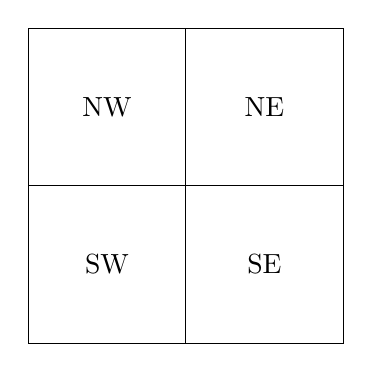
\begin{tikzpicture}
                \draw (1, 1) rectangle (3, 3);
                \draw (1, 3)rectangle (3, 5);
                \draw (3, 1)rectangle (5, 3);
                \draw (3, 3)rectangle (5, 5);
                \node at (2, 2){SW};
                \node at (4, 4){NE};
                \node at (2, 4){NW};
                \node at (4, 2){SE};
            \end{tikzpicture}
        }
        \caption{Квадратная матрица, разделенная на квадранты}
        \label{qmatrix}
    \end{minipage}
    \hfill
    % Second minipage
    \begin{minipage}[b]{0.45\textwidth}
        \centering
        \Tree [.Matrix
                [.NW [] ]
                [.NE [] ]
                [.SW [] ]
                [.SE [] ]
        ]
        \caption{Схематичное изображение одного из узлов дерева квадрантов и его потомков}
        \label{qtree1}
    \end{minipage}
\end{figure}


% !TeX spellcheck = ru_RU
% !TEX root = vkr.tex

\section{Постановка задачи}
Целью работы является исследование эффективности техники оптимизации \enquote{слияние ядер}, её возможности и ограничения применительно к деревьям квадрантов. Для её достижения были поставлены следующие задачи:
\begin{enumerate}
    \item Реализовать базовую функциональность: представление матрицы в виде деревьев квадрантов, поэлементные операции над ними, умножение.
    \item Применить технику реализации \enquote{слияние ядер} на template haskell для поэлементных операций над произвольным фиксированным количеством матриц и последовательного умножения и применения поэлементной операции.
    \item Произвести замеры производительности.
\end{enumerate}

% !TeX spellcheck = ru_RU
% !TEX root = vkr.tex

\section{Обзор}
В этом разделе будут введены необходимые для понимания работы термины и  понятия.
\subsection{Деревья квадрантов}
Деревья квадрантов~--- рекурсивная структура данных для представления разряженных матриц. Данная матрица приводится до квадратной с размером, равным степени двойки, далее,если все элементы матрицы равны, то дерево представляется в виде пары значения и размера и будет называться листом дерева, в ином случае разделяется на четыре равные части~--- дочерние узлы (квадранты), которые тоже представляют собой деревья квадрантов. Так происходит до тех пор, пока каждый узел не дойдёт до листа. Таким образом, строится дерево в привычном для математиков понимания этого слова. визуальное представление этого процесса представлено на рис. \ref{qmatrix} и рис. \ref{qtree1}. Эта структура позволяет \enquote{сжимать} повторяющиеся и находящиеся близко данные в один узел.
\begin{figure}[ht]
    \centering
    % First minipage
    \begin{minipage}[b]{0.45\textwidth}
        \centering
        \resizebox{\linewidth}{!}{
            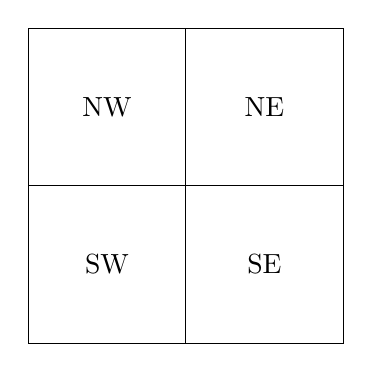
\begin{tikzpicture}
                \draw (1, 1) rectangle (3, 3);
                \draw (1, 3)rectangle (3, 5);
                \draw (3, 1)rectangle (5, 3);
                \draw (3, 3)rectangle (5, 5);
                \node at (2, 2){SW};
                \node at (4, 4){NE};
                \node at (2, 4){NW};
                \node at (4, 2){SE};
            \end{tikzpicture}
        }
        \caption{Квадратная матрица, разделенная на квадранты}
        \label{qmatrix}
    \end{minipage}
    \hfill
    % Second minipage
    \begin{minipage}[b]{0.45\textwidth}
        \centering
        \Tree [.Matrix
                [.NW [] ]
                [.NE [] ]
                [.SW [] ]
                [.SE [] ]
        ]
        \caption{Схематичное изображение одного из узлов дерева квадрантов и его потомков}
        \label{qtree1}
    \end{minipage}
\end{figure}

\subsection{Слияние ядер}
% Слияние ядер (англ. \textit{kernel fusion})
Требует уточнения
\subsection{Метапрограммирование}
Метапрограммирование~--- это процесс создание программ, которые в ходе своего выполнения генерируют другие программы. В контексте поставленной задачи оно было необходимо, так как нужно было
\begin{enumerate}[label=(\alph*)]
    \item генерировать функции в зависимости от данных, поданных пользователем;
    \item размер этого кода был довольно большим, но при этом обладал вполне регулярной структурой.
\end{enumerate}
В языке \Haskell{} есть встроенная библиотека с обширной и доступной документацией: \Th{}, которая позволяет генерировать код на \Haskell{} во время компиляции. При этом возможно использовать как синтаксис источника, так и более строгий специализированный для генерации кода.

% % !TeX spellcheck = ru_RU
% !TEX root = vkr.tex

\section{Метод}
В этом разделе будет показана идея оптимизации \enquote{слияние ядер} для деревьев квадрантов в деталях.
\subsection{Слияние ядер}
Основная идея данной техники заключается в том, чтобы за один проход по какой-либо структуре данных выполнять несколько независимых процессов в один, это позволяет избегать промежуточных структур данных, сразу генерируя результат. Применительно к линейной алгебре, если имеется несколько матриц $A = (a_{i, j}), B = (b_{i, j}), C = (c_{i, j})$ с одинаковыми размерностями $m \times n$ и поэлементная бинарная  операция $*$, то можно записать применение этой операции последовательно к матрицам как $\mathbf{map2} \ (*) \ (\mathbf{map2}\ (*)\ A \ B) \ C$, таким образом будет подсчитана промежуточная матрица $\mathbf{map2}\ (*)\ A \ B = (a_{i, j} * b_{i, j})$, иначе можно ввести функцию $\mathbf{map3}$, которая будет семантически совпадать с конструкцией $\mathbf{map2}\ (*) \ (\mathbf{map2}\ (*)\ A' \ B') \ C'$, но написать её таким образом, чтобы на каждом шаге подсчитывалось непосредственно $a_{i, j} * b_{i, j} * c_{i, j}$.

% !TeX spellcheck = ru_RU
% !TEX root = vkr.tex

\section{Реализация}
В данном разделе представлены некоторые технические подробности проделанной работы и ограничения, которые мешают проводить дальнейшую разработку без существенных изменений. Исходный код доступен по ссылке \url{https://github.com/KubEF/matrix-lib}
\subsection{Деревья квадрантов}
Для начала необходимо было реализовать базовую функциональность для работы с матрицами, представленными в виде деревьев квадрантов. Это рекурсивная структура данных, для задания таковых в \Haskell{} существует крайне удобное представление: алгебраические типы данных. Оно позволяет кратко записывать типы, которые будут являться одним из представителей.
\begin{lstlisting}[caption={пример конструирования односвязного списка над целыми числами}, language=Haskell, frame=single]
    data MyList Int = Nil | Cons Int (MyList Int)
\end{lstlisting}
Тип дерева квадрантов представлено в коде похожим образом
\begin{lstlisting}[caption={задание типа дерева квадрантов в библоитеке}, language=Haskell, frame=single, basicstyle=\ttfamily]
data QuadTree a =
    Leaf a Int
    | Node (QuadTree a) (QuadTree a) (QuadTree a) (QuadTree a)
\end{lstlisting}
В следствие такой структуры, реализовать поэлементные операции довольно просто~--- необходимо синхронно обходить деревья и применять операцию, когда дошли до листьев (если встретился узел и лист, то делим размер листа на два и так же спускаемся ниже). Умножение же на такой структуре данных работает схожим образом с обычными матрицами~\cite{10.1007/3-540-51084-2_9}:
\begin{gather*}
    \begin{bmatrix}
        NW_1 & NE_1 \\
        SW_1 & SE_1
    \end{bmatrix}
    \times
    \begin{bmatrix}
        NW_2 & NE_2 \\
        SW_2 & SE_2
    \end{bmatrix} = \\ =
    \begin{bmatrix}
        NW_1 \times NW_2 + NE_1 \times SW_2 & NW_1 \times NW_2 + NE_1 \times SW_2  \\
        SW_1 \times NW_2 + SE_1 \times SW_2 & SW_1 \times NE_2 + SE_1 \times SE_2
    \end{bmatrix}
\end{gather*}
Так что реализация умножения представляет собой синхронный обхода дерева с раздваиванием на каждом шаге.
\subsection{Генерация оптимизированного кода}
В случае последовательного применения поэлементных операций к $n$ деревьям возникают промежуточные структуры данных: результаты применения  бинарной операции к двум, которые передаются на вход следующей функции и не будут нужны в итоге.
Чтобы этого избежать, при помощи \Th{} генерируется код, который будет так же синхронно обходить не два, а, в общем случае, $n$ деревьев.
Этот подход позволит сразу создавать ответ без выделения памяти для промежуточных результатов.
\Th{} здесь необходим, так как он позволяет генерировать код по шаблону, а количество случаев, которые нужно обработать, растёт экспоненциально от $n$.

% Как-то переделать, чтобы было понятнее
Однако если попытаться оптимизировать связку умножения матриц с последующим применением поэлементной операции, то возникнут проблемы: в общем случае такой подход не работает.
Это происходит из-за того, что при отсутствии дистрибутивности поэлементной операции относительно \enquote{сложения}, которое определяет пользователь, невозможно делать синхронный разбор деревьев, поэтому будет необходимо посчитать промежуточную матрицу.
\subsection{Вывод}
В общем случае подход генерации \enquote{сливающего} кода, основанный на слиянии ядер, имеет необходимые ограничения, которые не позволяют соптимизировать умножение $n$ матриц и даже умножение двух матриц с последующим применением поэлементной операции.

% !TeX spellcheck = ru_RU
% !TEX root = vkr.tex

\section{Эксперимент}
\subsection{Цель эксперимента}
Целью эксперимента является сравнение оптимизированных версий функций с их неоптимизированными аналогами по времени исполнения.
\subsection{Условия эксперимента}
Разреженные матрицы были взяты из SuiteSparse Matrix Collection\footnote{SuiteSparse Matrix Collection: \url{http://sparse.tamu.edu/}. (дата обращения:   \DTMdate{2023-12-09}).} и представлены в таблице
\ref{used_matrixes}, где размер уже приведён к соответствующим степеням двойки для корректного построения дерева квадрантов.
%поправить и записать нормально размер
\begin{table}[h!]
    \rowcolors{2}{black!2}{black!10}
    \def\arraystretch{1.1}  % Растяжение строк в таблицах
    \setlength\tabcolsep{0.2em}
    \centering
    % \resizebox{\linewidth}{!}{%
    \caption{Использованные матрицы}
    \begin{tabular}[C]{l|
            c
            |r|r}
        \toprule
        Название &\multicolumn{1}{r|}{Размер}& Ненулевые элементы&\% заполненности  \\ \midrule
        meg4        ($Q_1$)& {$2^{13}$}\times{$2^{13}$} & 26324& 0,0766 \\
        aircraft    ($Q_2$)& {$2^{13}$}\times{$2^{13}$} & 20267 & 0,0718 \\
        fd12        ($Q_3$)& {$2^{13}$}\times{$2^{13}$} & 28462 & 0,0506 \\
        mc2depi     ($Q_4$)& {$2^{20}$}\times{$2^{20}$} & 2100225 & 0,0007 \\
        Hardesty2   ($Q_5$)& {$2^{20}$}\times{$2^{20}$} & 4020731 & 0,0014\\
        ecology1    ($Q_6$)& {$2^{20}$}\times{$2^{20}$} & 2998000 & 0,0002 \\
        webbase-1M  ($Q_7$)& {$2^{20}$}\times{$2^{20}$} & 3105536 & 0,0003\\
        \bottomrule
    \end{tabular}
    \label{used_matrixes}
\end{table}

Ниже представлены характеристики оборудования, на котором производились измерения.
\begin{verbatim}
    Operating System: Debian, unstable
    \end{verbatim}

\subsubsection*{CPU}
\begin{verbatim}
    Architecture:       x86_64
    Model name:         Intel(R) Core(TM) i7-4790 CPU @ 3.60
    \end{verbatim}

\subsubsection*{RAM}
\begin{verbatim}
    Total (Gi): 32
\end{verbatim}
Для измерений использовалась библиотека criterion\footnote{Criterion: \url{https://github.com/haskell/criterion}. (Дата обращения: \DTMdate{2023-12-10})}.

Были произведены замеры работы следующих функций:
\begin{itemize}
    \item measurement1 = $zipWithBinFunc4\ (+) \ Q_6 \ Q_6 \ Q_6\ Q_6$
    \item measurement2 = $zipWithBinFunc4\ (+) \ Q_5 \ Q_7 \ Q_5\ Q_6$
    \item measurement3 = $zipWith4Funcs\ (+) \ (*)\ (revDiv) \ Q_5 \ Q_7 \ Q_5\ Q_6$
    \item measurement4 = $map2\ revDiv\ (Q_3 \times Q_1)\ Q_2 $
\end{itemize}
Где $(+),\ (*), \ (revDiv) $ ~--- это операции сложения, умножения и обратного деления ($revDiv \ a \ b = b / a $) над вещественными числами соответственно, $\times$~--- операция умножения матриц над вещественными числами.
\begin{itemize}
    \item $map2$~--- функция, применяющая данную бинарную операцию элементам первой матрицы к элементам второй\\($A_{m\times n} = (a_{i, j}), \ B_{m\times n} = (b_{i, j}), \quad map2 \ (+)\ A \ B = (a_{i, j} + b_{i, j})$);
    \item $zipWithBinFunc4$~--- функция, эквивалентная последовательному применению $map2$ относительно одной и той же функции к данным четырём матрицам;
    \item $zipWith4Funcs$~--- функция, эквивалентная последовательному применению $map2$ относительно соответственно трёх переданных бинарных функций к четырём переданным матрицам.
\end{itemize}
\subsection{Результаты}
Результаты измерений представлены в таблице \ref{results}, где указано среднее время $\pm$ стандартное отклонение в секундах.
Оптимизированная версия на \Th{}, обычная версия на \Haskell{}.

\begin{table}[h!]
    \rowcolors{2}{black!2}{black!10}
    \def\arraystretch{1.1}  % Растяжение строк в таблицах
    \setlength\tabcolsep{0.2em}
    \centering
    % \resizebox{\linewidth}{!}{%
    \caption{Результаты измерений}
    \begin{tabular}[C]{l|
            *2{S
                        [table-figures-uncertainty=3, separate-uncertainty=true, table-align-uncertainty=true,
                            table-figures-integer=2, table-figures-decimal=3, round-precision=3,
                            table-number-alignment=center]
                }
        }
        \toprule
        Measurement num& \multicolumn{1}{r}{\Th/с}& \multicolumn{1}{r}{\Haskell/с} \\ \midrule
        measurement1 & 1.050 \pm 0.081 & 2.530 \pm0.118   \\ \midrule
        measurement2 & 4.010 \pm 0.425 & 7.370 \pm0.001  \\ \midrule
        measurement3 & 2.280 \pm 0.001 & 4.570 \pm  0.447  \\ \midrule
        measurement4 & 74.200 \pm 0.460  & 76.700 \pm  0.071   \\
        \bottomrule
    \end{tabular}
    \label{results}
\end{table}

Анализируя полученные данные, можно заключить, что оптимизация позволила значительно, почти в 2 раза, сократить время работы программы для поэлементных операций.

% !TeX spellcheck = ru_RU
% !TEX root = vkr.tex

\section*{Заключение}
В рамках проделанной работы получены следующие результаты:
\begin{enumerate}
    \item Реализована библиотека для работы с матрицами, представленными в виде деревьев квадрантов с базовой функциональностью.
    \item Написаны оптимизированные с помощью техники слияние ядер функции применения поэлементных операций для $n$ матриц.
    \item Проведены измерения, показывающие, что техника оптимизации даёт существенный результат.
\end{enumerate}
Дальнейшая работа заключается в поиске путей обхода или обработки выявленных в ходе работы ограничений. Предположительно, написать предметно-ориентированный язык для линейной алгебры и дистиллятор для него.


\setmonofont{CMU Typewriter Text}
\bibliographystyle{ugost2008ls}
\bibliography{vkr}
\end{document}
